% Interpretations: what do the results mean?
% Implications: why do the results matter?
% Limitations: what can’t the results tell us?
% Recommendations: what practical actions or scientific studies should follow?

Section \ref{section:ExperimentComparisonTimeLengths} reveals, that the 2h time length (from the 3h dataset) produced the most distinct and well defined clusters, according to the average Silhouette Coefficient, Davies-Bouldin Index, and Caliński-Harabasz Index results. The 1h time length (from the 3h dataset) came second, and the 30 min time delta (from the 1h dataset) came third. When considering the highest number of evaluation score "wins" over different t-SNE and clustering results, the 30 min time delta (from the 1h dataset) however came top, followed by the 1h time length (from the 3h dataset) and then the 2h time length (see figure \ref{figure:clusteringResultsGraphTotal}). It can therefore be concluded, that these 3 time deltas are the best performers.

The 45 minute time delta in the 1 hour data files performed the lowest, with 0 wins. The fact that 45 never out performed the other time lengths shows consistency, despite the different results. 1h 30 min (3h), 1h (1h), 2h 30 min (3h) and 3h (3h) all had no more than 2 wins. 


\begin{figure}
  \centering
  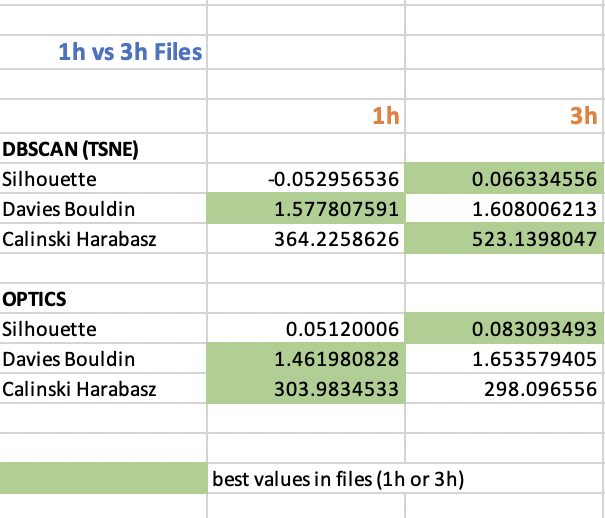
\includegraphics[width=0.5\textwidth]{./images/clusteringResults/clusteringResults7.png}
  \caption{Evaluation scores comparison from averaged 1h and 3h dataset runs+ of t-SNE and clustering.}
  \label{figure:clusteringResults7}
\end{figure}


The results from \textcite{AboutToEat2016Rahman} (as mentioned in section \ref{section:RelatedWork}) showed, that higher time lengths (e.g. 100 minutes) performed better than shorter ones. They deducted, that smaller window sizes were susceptible to noise and had a higher gap between precision (exactness) and recall (completeness). 
% Coarser ones however were unable to detect recent events, though performed better in the comparison of precision and recall.
This discovery could also apply to the results of this experiment, considering that the 2h and 1h time lengths in the three hour data files were under the top 3 results.


To determine whether the 1 hour or 3 hour aggregation files led to better clusters, the average results of both time files are compared in figure \ref{figure:clusteringResults7}. Both the 1h and 3h datasets have the same amount of wins. When scanning other comparisons of these files (also the ones utilised for finding the t-SNE parameters), it is noticeable, that the 1h and 3h datasets either have the same number of wins, or the 3h dataset has more. This indicates that overall, the three hour aggregation files produce more superior clusters.

Of the 36 number of wins across all time deltas (the 1h and 3h aggregation files combined), 14 of these were achieved by the 1h data file time lengths (38.9\%), the other 22 by the 3 hour dataset (61.1\%). A possible explanation, as to why the 3h dataset might have created better clusters, was that the dataset had more rows. After the data preparation step, the 1h aggregation set was left with an average (depending on number of time length columns considered) of 1654 rows, whilst the 3h set was left with over double the amount of rows with an average of 3976.5 rows. The use of more data could have resulted in more similar rows and more improved clusters. Another aspect to consider, is that shorter sensor data recorded for shorter time lengths might not be long enough to detect underlying stress patterns.

Moreover, the higher the number of rows, the more robust the clusters could be towards potential outliers. As explained in section \ref{section:silhouetteCoefficient}, the Silhouette Score compares the within cluster distances to the distance of a neighbouring cluster. If many points are well placed within a cluster, an outlier will have little impact against the many short distances. However, if the cluster is not very dense and only contains a few "good" assigned data points, an outlier could have a larger impact on the result.





%e.g. fight or flight https://humanstress.ca/stress/what-is-stress/history-of-stress/


% This is stress resulting from specific events or situations that involve novelty, unpredictability, a threat to the ego, and leave us with a poor sense of control N.U.T.S. This ‘on the spot’ type of stress can be good for you because the stress hormones released help your mind and body to deal with the situation.

% i.e.: Almost getting into a car accident or giving a speech in front of people. You feel your heart beat in your throat, you become hyper aware of everything around you, and feel pumped. These are signs that your stress hormones are hard at work!
In order to provide Just-in-Time Intervention, the SmartEater app would need to predict upcoming stress. There are different types of stress. The Canadian Centre for Studies on Human Stress (CSHS) \footnote{\url{https://humanstress.ca/stress/understand-your-stress/acute-vs-chronic-stress/}} differentiate acute and chronic stress. Acute stress is caused by a particular event or setting, when something is new and feels out of control. For example like a presentation in front of people. Chronic stress is longer term and caused by repeated situations that cause stress. The data points would need to account for and recognise these different types of stress. For example, if stress is short, then a longer time delta will likely make it seem less relevant, compared to all the unstressed data. However, if it is long, a shorter time delta might miss it or only perceive a small part of it. This could lead to false cluster assignments or noise. However, it could also create its own clusters. This could also be a reason why middle time lengths, such as 2h, 1h (3h data files) created more distinct clusters, since it may have been more likely to recognise these differences. The fact that there was not one specific time length that always performed higher than the others shows, that a single time length may not be enough to be able to create clear clusters. Different time lengths might be needed to detect different patterns.

When visually comparing the clusters in appendix \ref{appendix:clusteringResults}, the 3h datasets appear to be denser, whilst the 1h datasets have more wider non-populated regions between clusters. The 1h dataset top performer, 30 minutes, seems to be scattered in a slightly different shape to the other scatter plots of the 1h dataset. It appears to be spread out wider along the x axis, similar to the scatter plots from the 3h data files. The 30 minute time length achieved the highest number of wins in the 1h dataset. It could be argued, that the shape of the scattering of the points with similarity to the 3h data scatter plots, that also performed well, could be an indicator for more enhanced clustering results.


For future work, it might be advisable to get more data from users for a longer period of time. However, it would also be necessary confirm that the clusters were created for stress levels and not for each user (since users behaviour could exhibit similarities). As implemented in this thesis, this could be achieved by highlighting each user's results with a unique colour. It might also be beneficial to support the mathematical evaluations with hand drawn clusters found by test users in user studies. Especially since the scores are different each time t-SNE is computed, sometimes leading to different results. As mentioned in section \ref{section:TheoryDataMining} by \textcite{DataMiningAndPredictiveAnalytics}[9], data mining requires continuous human supervision for quality monitoring and evaluation.


% As stated by \textcite{DataMiningAndPredictiveAnalytics}[9-13, 15-16], data mining requires continuous human supervision for quality monitoring and evaluation. Software alone will serve wrong results. Data mining is used for description of patterns and trends, estimation of numerical values, prediction of future results, classification of categorical variables, clustering of similar objects and association of attributes. 
% in section \ref{section:TheoryDataMining} they say about how need constant human supervison - for this reason didn'T fully trust numbers
% The fact however, that there might not be one specific time delta that is most suitable across all users.

% The time lengths that average multiple columns could create rows with more values, .
% maybe more columns - made the data more different in higher - but too high too different more scattered

% For future work, it might be advisable to get more data from users for a longer period of time. However, it would also be necessary confirm that the clusters were created for stress/not stress and for each user (since users behaviour could exhibit similarities). It might also be beneficial to support the mathematical evaluations with hand drawn clusters found by test users in user studies. Especially since the scores are different each time t-SNE is computed, sometimes leading to different results.

%todo: especially since the maths evaluation score

% higher amount of rows - more robust to outliers

 

% 30 min performed well in both aggregations



%1: 1. Adam, T.C., Epel, E.S.: Stress, eating and the reward system. Physiology & behavior 91(4), 449–458 (2007)
%21: 21. Schwabe, L., Dickinson, A., Wolf, O.T.: Stress, habits, and drug addiction: a psychoneuroendocrinological perspective. Experimental and clinical psychopharmacology 19(1), 53 (2011)





%1h-1: 1681, 3h-1: 3949
%1h-2: 1655, 3h-2: 3987
%1h-3: 1650, 3h-3: 3967
%1h-4: 1630, 3h-4: 3951
%----------, 3h-5: 3993
%----------, 3h-6: 4012
%----------------------
%averages:
%----------------------
%
%
%


% Naturally, this reduced the total number of rows left. As an example, the number of rows left for the 1h data files only using the first feature columns (15 min) was 1681 from initial 8283 (20.29\%). In the 3h dataset (first column, 30 min) only 3949 from 14091 rows remained (28.02\%).










% CHAIN ARGUMENTATION, e.g. explain why data from the same person could be together
% Answer research question by creating hypothesis (which i don't have to answer though)

% can also see, when was comparing perplexity, learning rate - the 3h files mostly had the better values
% Spalten wie NOTIF, SCRN, APP.. haben sehr oft 0 und sind auch teilweise von einander abhängig. Z.B. Wenn SCRN ausgeschaltet ist, ist in den meisten Spalten auch LIGHT, die APP Spalten und auch oft NOTIF 0. NOTIF ist generell sehr oft 0, weil man nicht ständig Notifikationen bekommt. LIGHT ist die Umgebungslicht. Oft wenn man das Handy nicht benutzt, hat man es in eine Tasche. Aus diesem Grund gibt es sehr viele ähnliche Spalten. (Ich habe auch nachgeschaut welche Spalten in diese Schleife sind und es sind fast immer solche (außer ein paar Ausreßer)).
% Weiters kann man sehen, wenn SCRN 0 ist und es gibt Notifikationen, dann gibt es auch bei einer der APP Spalten Aktivität. Od ab und zu, wenn der SCRN angegangen ist, dann zeigt auch eine APP Aktivität.

% Warum die Schleife noch da war, wie nur die AUDIO und ACC Spalten verwendet werden, ist vermutlich deshalb, weil die Accelerometer Werte auch sehr ähnlich waren. Beim Untersuchen der Tabelle, wo nur diese zwei Spalten verwendet wurden ist aufgefallen, dass mehr als 50% der ACC Werte zwischen in ein Intervall von 0.1 (z.B. zwischen 0.2 & 0.3) lagen, obwohl die ACC Werte in dem Bespiel insgesamt eine Spannungsbreite von 7.89069115 Werte (z.B. zw. 0 & 7.89069115) einnahmen.

% Man sieht auch, dass öfters die Punkte von der gleichen Test Person gemeinsam „angehäufelt“ sind. Dies könnte sich vielleicht erklären lassen, dass die Daten einer Testperson ähnlich sind, weil er/sie die ähnlichen Handlungen machen (z.B. ähnliche schnelle Bewegungen, ähnliche Lautstärke, …)





% (Future): look over in more detail? or other evalutation methods, or also human look over


% \textbf{todo: finish}
